\documentclass{article}
\usepackage[english]{babel}
\usepackage{longtable}
\usepackage[top=1in, bottom=0.25in, left=1.25in, right=1.25in,includefoot,heightrounded]{geometry}
\usepackage{indentfirst}
\usepackage[utf8]{inputenc}
\usepackage{amsmath,amssymb}
\usepackage{graphicx,tikz}
\usepackage{hyperref}
\usepackage[colorinlistoftodos]{todonotes}
\usepackage[document]{ragged2e}
\usepackage{fancyhdr}
\usepackage{enumerate}
\usepackage{listings}
\usepackage{color}
\usepackage{flowchart}
\usepackage{hyperref}
\usepackage{graphicx}
\usetikzlibrary{arrows}

\usetikzlibrary{shapes.geometric, arrows}
\tikzstyle{startstop} = [rectangle, rounded corners, minimum width=3cm, minimum height=1cm,text centered, draw=black, fill=red!30]
\tikzstyle{decision} = [diamond, minimum width=4cm, minimum height=0.5cm, text centered, draw=black, fill=green!30]
\tikzstyle{process} = [rectangle, minimum width=3cm, minimum height=1cm, text centered, draw=black, fill=orange!30]
\tikzstyle{arrow} = [thick,->,>=stealth]
\tikzstyle{io} = [trapezium, trapezium left angle=70, trapezium right angle=110, minimum width=2cm, text width=4cm, minimum height=1cm, text centered, draw=black, fill=blue!30]

\pagestyle{fancy}
\fancyhf{}
\lhead{Myles Deslippe}
\rhead{Comp 3670 | Computer Networks}
\cfoot{\thepage}

\definecolor{MyDarkGreen}{rgb}{0.0,0.4,0.0}
\lstset{inputencoding=ansinew}
\lstset{breaklines=true} 

\begin{document}

    \section*{\centering{Wireless Networks}}

    \subsection*{Wireless Network Introduction}
    \begin{itemize}
        \item A \textbf{wireless host} is a \textbf{network host} that communicates \textbf{wirelessly}. Such devices may be stationary or mobile.
        \item A \textbf{base station} is a \textbf{transmission and reception station} that is located in a \textbf{fixed location} and serves as a \textbf{central connection point} for \textbf{wiresless devices} to \textbf{communicate}.
        \begin{itemize}
            \item They are usually \textbf{connected to a wired network}, and relay \textbf{packets} between \textbf{wireless devices} and \textbf{devices on the wired network}.
            \item An example is cellular towers.
        \end{itemize}
        \item A \textbf{wireless link} is a \textbf{link} that is used to \textbf{connect wireless hosts} to \textbf{base stations}.
        \begin{itemize}
            \item They have different acces protocols to coordinate link access, and can have various transmission rates, distances, and frequency bands.
        \end{itemize}
        \item Types of wireless links, and their ranges:
        \item[] 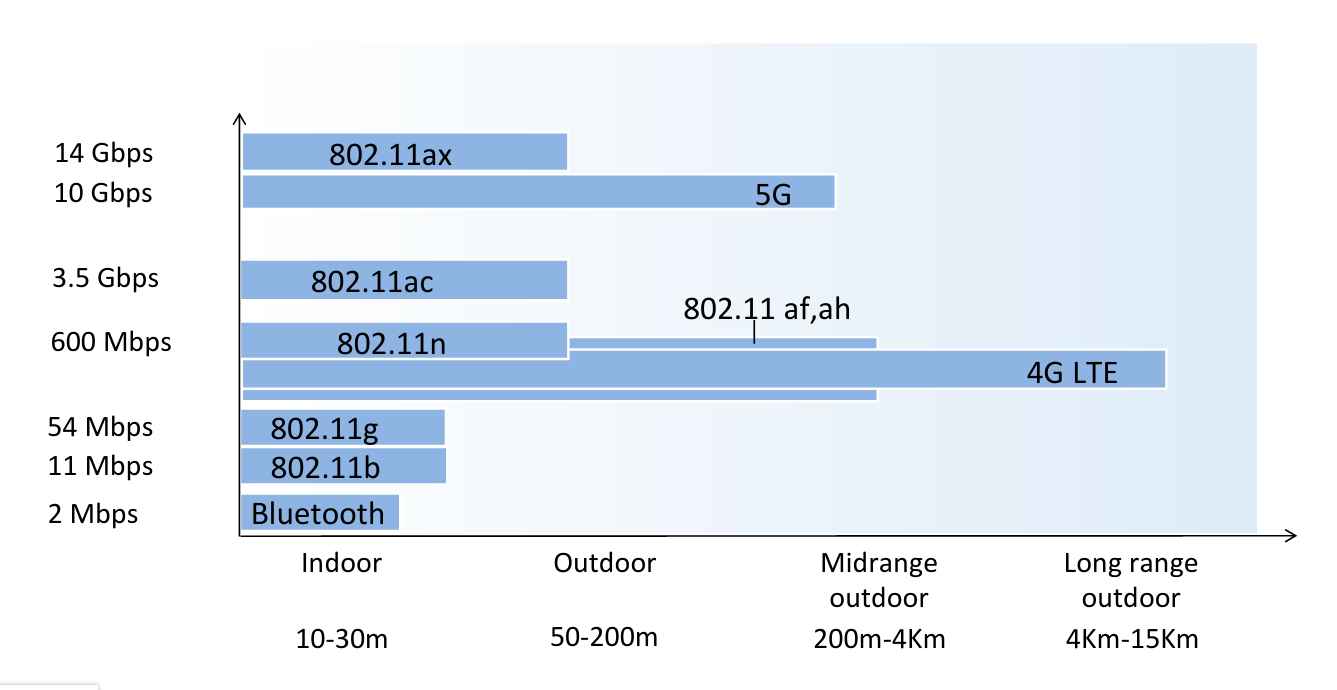
\includegraphics[width=\textwidth - 25pt]{images/Wireless-Links.png}
        \item A \textbf{handoff} occurs when a \textbf{mobile device changes from one base station to another}. 
        \item \textbf{Wireless network modes}:
        \begin{enumerate}
            \item \textbf{Infastructure mode} is when a \textbf{base station connects mobile devices, to wired networks}.
            \item \textbf{Ad hoc mode} is when there are \textbf{no base stations, nodes can only transmit wirelessly to each other}.
        \end{enumerate}
    \end{itemize}

    \subsection*{Wireless Network Characteristics}
    \begin{itemize}
        \item As the \textbf{distance increases} between \textbf{wireless nodes}, the \textbf{signal strength of the link decreases}.
        \item There can be \textbf{interference from other sources} if a lot of \textbf{wireless links} are in the \textbf{same area}.
        \item \textbf{Multipath propagation occurs}; radio signals reflect off of objects and arrive at the destination at slightly different times.
        \item Overall, \textbf{wireless communication} is much \textbf{more difficult} than \textbf{wired communication}.
        \item \textbf{Signal-To-Noise Ratio (SNR)} is one way measure \textbf{interference}.
    \end{itemize}

    \subsection*{Code Division Multiple Access (CDMA)}
    \begin{itemize}
        \item \textbf{Code Division Multiple Access (CDMA)} consits of \textbf{assigning a unique code} to \textbf{each user}. All users \textbf{communicate over the same frequency}, but \textbf{each user} has a \textbf{"chipping" sequence} to \textbf{encode data}.
        \item If \textbf{codes are "orthogonal"} it allows \textbf{multiple users} to \textbf{coexist and transmit simultaneously} with \textbf{minimal interference}.
    \end{itemize}

    \subsection*{802.11 Wireless Local Area Networks (Wi-Fi)}
    \begin{itemize}
        \item The \textbf{802.11 LAN architecture} consists of \textbf{wireless hosts} communicating with a \textbf{base station}.
        \item \textbf{Base stations} are referred to as \textbf{Access Points (AP)}.
        \item The \textbf{802.11 frequency spectrum} is divided into \textbf{channels at different frequencies}. The access point admin chooses the frequency for each access point (interference is possible).
        \item New \textbf{arriving hosts} must \textbf{associate with an access point}. They do this by scanning channels and listening for beacon frames containing the access point's service set identifier (SSID) and MAC address. After they receive the beacon frames, they can choose an access point to associate with.
        \item Some \textbf{access points} require \textbf{authentication} inorder for \textbf{wireless hosts to connect}.
        \item \textbf{Access points} have an internal \textbf{DHCP server}, allowing them to assign \textbf{ip addresses} to \textbf{wireless hosts}.
        \item There are \textbf{two ways} that \textbf{arriving hosts} can \textbf{scan for access points}:
        \begin{enumerate}
            \item \textbf{Passive Scanning} | The wireless host listens for beacon frames, sends an association request frame, and waits for an association response frame.
            \item \textbf{Active Scanning} | The wireless host broadcasts a probe request, probe responses are sent back from access points, the wireless host then sends a request frame to the access point it wants to associate with, and waits for a response frame.
        \end{enumerate}
        \item \textbf{CSMA/CA} is used to detect collision. If the sender detects that the channel is idle, they will send the entire frame. If the sender detects that the channel is busy, it will start a random backoff time and wait to transmit. After transmission the sender will wait from an ACK response, if it does not receive the response, the frame is retransmitted.
        \item \textbf{802.11 frames} consist of \textbf{9 parts}:
        \begin{enumerate}
            \item \textbf{Frame Control} | Bit flags.
            \item \textbf{Duration} | The duration of reserved transmission time.
            \item \textbf{Address 1} | The MAC address of the wireless host or access point receiving the frame.
            \item \textbf{Address 2} | The MAC address of the wireless host or access point transmitting the frame.
            \item \textbf{Address 3} | The MAC address of the router interface to which the access point is attached to.
            \item \textbf{Sequence Control} | The frame sequence number for reliable data transmission.
            \item \textbf{Address 4} | An address that is reserved for use in ad hoc mode.
            \item \textbf{Payload} | The encapsulated datagram.
            \item \textbf{CRC}
        \end{enumerate}
        \item[] 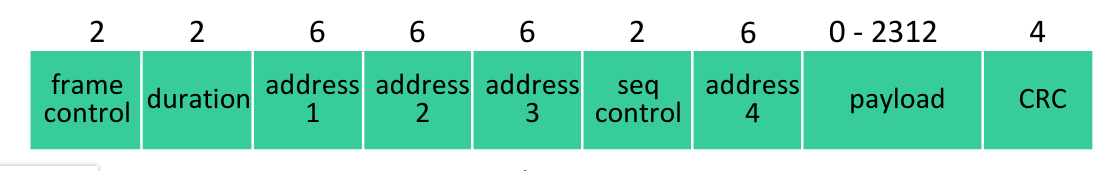
\includegraphics[width=\textwidth - 25pt]{images/WiFi-Frame.png} 
    \end{itemize}

    \subsection*{Bluetooth}
    \begin{itemize}
        \item \textbf{Bluetooth} is a \textbf{short-range, wireless technology} that is used for \textbf{transmitting data} between \textbf{fixed and mobile devices over short distances}.
        \item \textbf{Bluetooth} is \textbf{ad hoc}; it has \textbf{no Infastructure}.
        \item \textbf{Bluetooth} uses a \textbf{2.4-2.5 GHz ISM radio band} and can transmit up to \textbf{3Mbps}.
        \item \textbf{Bluetooth clients} can \textbf{"go to sleep" (park)} and \textbf{wakeup later} to \textbf{preserve battery}. This is known as \textbf{parked mode}.
        \item \textbf{Bluetooth} uses \textbf{bootstrapping}. \textbf{Nodes self-assemble into piconet}.
    \end{itemize}

    \subsection*{4G/5G Cellular Networks}
    \begin{itemize}
        \item \textbf{Cellular networks} are the \textbf{solution} for \textbf{wide-area mobile networks}. Such networks have a \textbf{transmission rate} of up to \textbf{100s of Mbps}.
        \item \textbf{Cellular networks} are \textbf{interconnected to the wired internet}.
        \item \textbf{Cellular devices} are identified via \textbf{Subscriber Identity Module Cards (SIM Cards)}.
        \item Unlike the \textbf{wired-internet}, in \textbf{cellular networks}, \textbf{mobility} is treated as a \textbf{first class service}.
        \item \textbf{LTE} introduced a \textbf{seperation} between the \textbf{control plane} and the \textbf{data plane}. \textbf{LTE} introduced \textbf{new protocols} for \textbf{mobility managment, security, and authentication} on the control plane. \textbf{LTE} introduced \textbf{new protocols} at the \textbf{link and physical layer} aswell.
    \end{itemize}

\end{document}